A large part of the design of a legged robot depends on the design of a simple leg - more specifically the degrees of freedom that a single leg has. The degrees of freedom that a single leg has is determined by the amount of dimensions that the leg can make a controlled movement in, independently from any other dimensions. There are two common underlying designs in robot leg design - these are for two and three degrees of freedom respectively.\\

Figure \ref{fig:2DOF} shows an example of a common design that has two degrees of freedom. The design therefore contains two joints in one leg. In this example, the first joint is positioned vertically to form the hip op the robot leg. This allows for the side-to-side motion required for walking. The second joint is positioned horizontally to allow the lowest limb to move up and down. The two degrees of freedom controlled by this leg design is therefore the horizontal angle of the leg and the height of the foot. These two (and only these two) parameters can therefore be controlled completely independently.
\FloatBarrier
\begin{figure}[h]
\centering
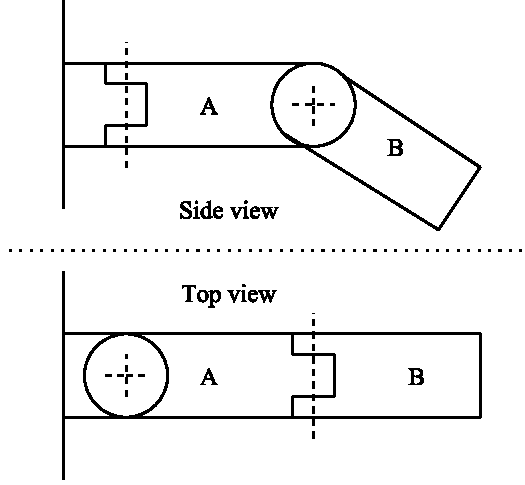
\includegraphics[scale = 1]{pics/2DOF.pdf}
\caption{Example of a leg design with two degrees of freedom.}
\label{fig:2DOF}
\end{figure}
\FloatBarrier
An example of a robotic leg with three degrees of freedom can be seen in Figure \ref{fig:3DOF}. This design is similar to that of the leg with two degrees of freedom seen in Figure \ref{fig:2DOF}, with the only addition being a second horizontal joint further down from the first. This additional limb means that the horizontal distance from the foot to the hip can be controlled as well as the height of the foot. These two controlled parameters, together with the horizontal leg angle which can also be controlled independently as in the case of the two degrees of freedom design, means that this design has a total of three degrees of freedom.
\FloatBarrier
\begin{figure}[h]
\centering
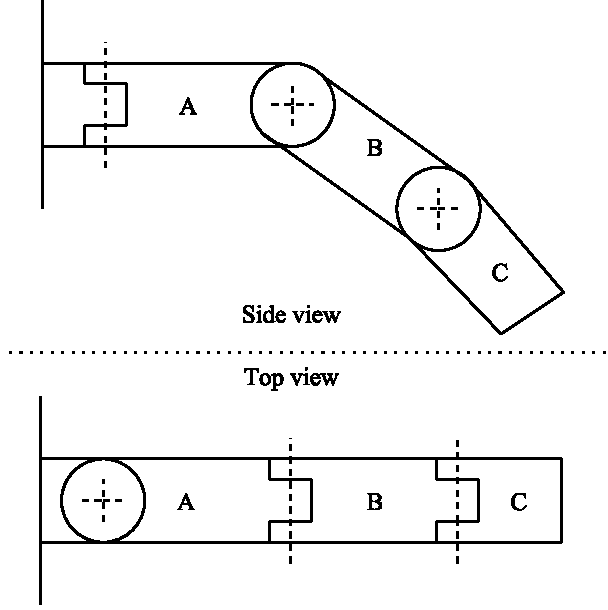
\includegraphics[scale = 1]{pics/3DOF.pdf}
\caption{Example of a leg design with three degrees of freedom.}
\label{fig:3DOF}
\end{figure}
\FloatBarrier


The design with three degrees of freedom has the advantage of being able to lift a leg without altering the horizontal position of the leg. This means that the robot is able to walk without altering the height of the body of the robot. The robot is therefore able to cross rougher terrain much better because of the ability to alter the height of the robot feet as the terrain requires. With the design that has two degrees of freedom, the foot height is a function of the horizontal extension of the leg. With this design the main advantage is the simplicity - both mechanically and in software. The cost and power consumption will also be much lower because of the reduced amount of actuators.\\

Due to the much greater flexibility of the design with three degrees of freedom and the ability to cross rougher terrain, this will be the platform implemented in the final design.\\